\chapter{The Dynamic Grid}\label{ch:dynamicGrid}
% \def\alfPlusEps{\alpha}
% \textit{Often in math, you should view the definition not as a starting point, but as a target. Contrary to the structure of textbooks, mathematicians do not start by making definitions and then listing a lot of theorems, and proving them, and showing some examples. The process of discovering math typically goes the other way around. They start by chewing on specific problems, and then generalising those problems, then coming up with constructs that might be helpful in those general cases,and only then you write down a new definition (or extend an old one). - Grant Sanderson (AKA 3Blue1Brown) https://youtu.be/O85OWBJ2ayo?t=359}
This chapter provides an extended summary to the paper ``Dynamic grids for Finite-Difference Schemes in Musical Instrument Simulations'' \citeP[G]. The paper presents a novel method to smoothly add and remove grid points from a FD scheme, which allows for dynamic parameter variations without compromising stability or quality of the simulation (see Section \ref{sec:quality1DWave}). 

After a brief introduction, this chapter summarises paper \citeP[G] and extends it by providing details on the implementation of the displacement correction and the modal analysis shown in the paper. This chapter continues by providing additional results of various experiments to substantiate choices made in the paper. Finally, this chapter lists several examples of potential future use cases for the method presented here. 

\section{Background and motivation}
Simulating musical instruments using physical modelling -- as mentioned in Chapter \ref{ch:physMod} -- allows for manipulations of the instrument that are impossible in the physical world. Examples of this are changes in material density or stiffness, cross-sectional area (strings, acoustic tubes), thickness (membranes, plates) and size of the system in general. Using FDTD methods to discretise PDEs, constrains the simulation to a grid of a finite amount of points. As explained in Section \ref{sec:quality1DWave}, the definition of this grid ties the parameters set by the user to the stability and quality of the simulation, making FDTD methods extremely inflexible to parameter changes. 

Apart from being potentially sonically interesting, dynamic parameter changes also happen in the real world. A prime example is the trombone published in paper \citeP[H] using the method presented here. A collection of examples for potential future use cases of the method are listed in Section \ref{sec:examples}.

\section{Extended summary}
This section summarises the \textit{dynamic grid method} presented in paper \citeP[G] and extends the paper by providing details on the implementation. 

\subsection{Problem statement}
Consider the 1D wave equation  as presented in Section \ref{sec:1DWave}, describing the motion of a system of length $L$ (in m), its state is denoted by $q = q(x,t)$, and is defined for $t\geq 0$ and $x\in\D$ with domain $\D = [0, L]$. This state variable can be discretised to a grid function $\qln$ with $n\in \mathbb{N}^0$ and $l \in \{0, \hdots, N\}$, where $N$ is the number of intervals between the grid points. The PDE in Eq. \eqref{eq:1DwavePDE} (using state variable $q$) can then be discretised to the following FD scheme:
\begin{equation}\label{eq:1DWaveDynamic}
    \dtt \qln = c^2\dxx \qln.
\end{equation}
If one would like to dynamically vary the wave speed $c$, several issues arise. Performing the usual calculations for the number of intervals $N$, Courant number $\lambda\leq 1$ and grid spacing $h$ (Eq. \eqref{eq:orderOfCalc}),
\begin{equation}\label{eq:dynamicOrderOfCalc}
    h := ck, \quad N := \floor[\frac{L}{h}], \quad h := \frac{L}{N}, \quad \lambda := \frac{ck}{h},
\end{equation}
shows that a change in $c$ can cause abrupt changes in $N$ due to the flooring operation. One could avoid this issue by fixing $N$ at the start of the simulation and decrease $c$, i.e., tune it away from the stability condition. The issue here, is that the simulation quality and bandwidth decreases very rapidly as explained in Section \ref{sec:quality1DWave}. 

Paper \citeP[G] proposes a \textit{fractional} number of intervals $\Nfrac$, where $N = \floor[\Nfrac]$, such that grid points could potentially be added and removed from the grid without causing artefacts. As the number of intervals is fractional, the flooring operation in Eq. \eqref{eq:dynamicOrderOfCalc} can be removed, and $h$ does not have to be recalculated. Equation \eqref{eq:dynamicOrderOfCalc} can be changed to
\begin{equation}\label{eq:newOrderOfCalc}
    h:= ck, \quad \Nfrac := \frac{L}{h}, \quad \lambda := \frac{ck}{h},
\end{equation}  
which results in that the stability condition is always satisfied with equality. Issues regarding simulation quality and bandwidth could thus be resolved. In the following, the variables $c$, $h$, $\Nfrac$ and $N$ will receive a superscript $n$ as they are time-varying.

\subsection{Splitting the scheme}
Rather than working with the scheme in Eq. \eqref{eq:1DWaveDynamic} directly, paper \citeP[G] proposes to split it into two separate subsystems, according to
\begin{subequations}\label{eq:splitFDS}
    \begin{align}
        \dtt \ulun &= (c^n)^2\dxx \ulun,\\
        \dtt \wlwn &= (c^n)^2\dxx \wlwn,
    \end{align}
\end{subequations}
where $l_u \in \{0, \hdots, M^n\}$ and $l_w \in \{0, \hdots, M_w^n\}$ and integers 
\begin{equation}
    M^n =\ceil[0.5 N^n] \qaq M_w^n =\floor[0.5 N^n]
\end{equation}
are the number of intervals between grid points of each respective subsystem. This yields a total of $M^n + M_w^n + 2$ grid points, which is one more than the original scheme in Eq. \eqref{eq:1DWaveDynamic}. Paper \citeP[G] shows that this system can be shown to exhibit identical behaviour to the original system, using the boundary conditions described shortly.

\subsubsection{Locations of grid points}
The schemes in Eq. \eqref{eq:splitFDS} are placed on the same domain $x$, where the left boundary of $\ulun$ and the right boundary of $\wlwn$ -- referred to as the \textit{outer boundaries} -- are placed at the following locations:
\begin{equation}\label{eq:outerBoundaries}
    x_{u_0}^n = 0, \quad x_{w_{M_w^n}}^n = L.
\end{equation}
Here, $x_{q_l}^n$ is the location of grid point $q_l$ (in m from the left boundary) at time index $n$.

The right boundary of $u$ and the left boundary of $w$ -- referred to as the \textit{inner boundaries} -- are placed at the following locations:
\begin{equation}\label{eq:innerBoundaries}
    x_{u_{M^n}}^n = M^nh^n, \quad x_{w_{0}}^n = L-M_w^nh^n.
\end{equation}
If $\Nfrac^n$ is an integer, the inner boundaries perfectly overlap (see Figure \ref{fig:twoFreeStrings}). If the wave speed $c^n$ changes, which consequently changes $h^n$ according to Eq. \eqref{eq:newOrderOfCalc}, the outer boundaries will remain at their respective locations given by Eq. \eqref{eq:outerBoundaries} and all other grid points will move to or from the outer boundary of their respective system according to\footnote{Notice that Eq. \eqref{eq:hLocs} applies to all grid points, and includes the definitions for the outer and inner boundaries in Eqs. \eqref{eq:outerBoundaries} and \eqref{eq:innerBoundaries}.} 
\begin{equation}\label{eq:hLocs}
    x_{u_{l_u}}^n =l_uh^n, \quad x_{w_{l_w}}^n = L-(M_w^n-l_w)h^n.
\end{equation}
See Figure \ref{fig:twoFreeStringsGridMove}. As an example, if $c^n$ decreases, $h^n$ decreases, causing all grid points of system $u$ to move towards the left boundary and all grid points of system $w$ to move towards the right boundary (except for grid points at the outer boundaries).

The distance between the inner boundaries is expressed as the fractional part of $\Nfrac^n$
\begin{equation}\label{eq:alphaDef}
    \alpha = \alpha^n = \Nfrac^n - N^n
\end{equation}
and essentially states how many times the grid spacing $h^n$ can fit between the inner boundaries, which is always less than once (see Figure \ref{fig:twoFreeStringsGridZoomed}). If the value of $N^n$ changes, a grid point will be added to or removed from the grid as will be shown in Section \ref{sec:addRemove}.

\def\figwidth{0.9}
\begin{figure}[t]
    \centering
    \subfloat[]{\label{fig:twoFreeStrings}{ 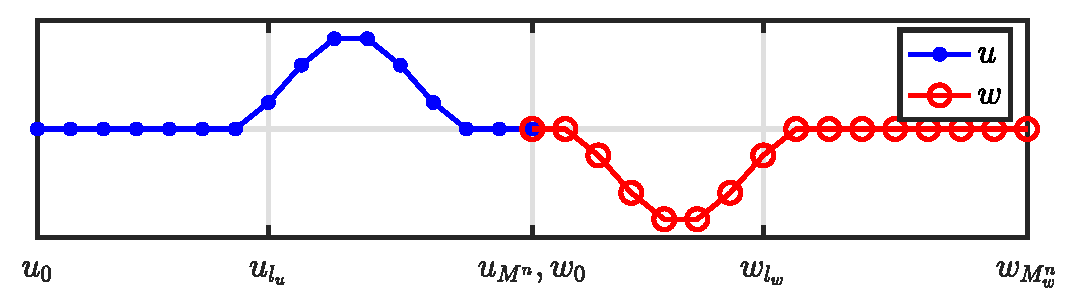
\includegraphics[width=\figwidth\textwidth]{figures/contributions/dynamicgrid/twoFreeStringsNarrow.eps}}}\\
    \vspace{-1em}\subfloat[]{\label{fig:twoFreeStringsGridMove}{ 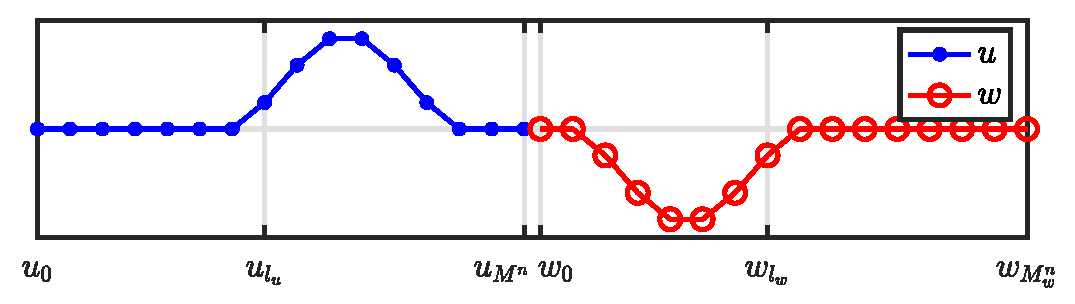
\includegraphics[width=\figwidth\columnwidth]{figures/contributions/dynamicgrid/twoFreeStringsGridMoveNarrow.eps}}}\\
    \vspace{-1em}\subfloat[]{\label{fig:twoFreeStringsGridZoomed}{ 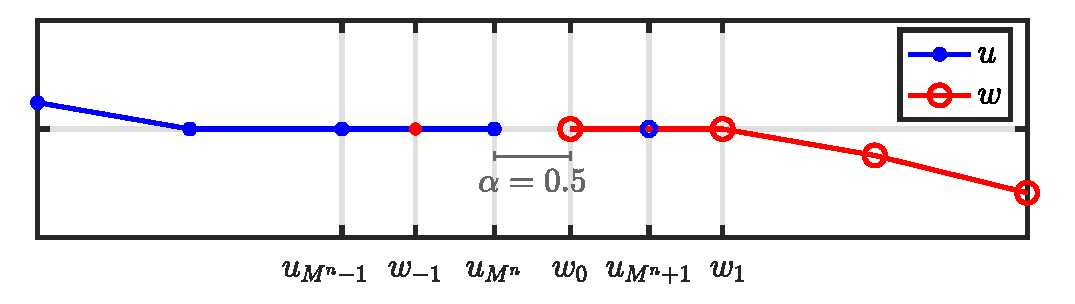
\includegraphics[width=\figwidth\columnwidth]{figures/contributions/dynamicgrid/twoFreeStringGridMoveZoomedNarrow.eps}}}
    \vspace{-1em}\caption{ Illustration of the proposed method. In all figures, the x-axis shows the location of the respective grid points%(fx. $x_{u_l^n}$)
    , but `$x^n$' is omitted for brevity. (a) Locations of the states of two (1D wave) systems connected at the inner boundaries ($\Nfrac^n = 30$, $x_{u_{M^n}}^n = x_{w_0}^n$). (b) When $c^n$, and consequently $h^n$, are decreased and the positions of the grid points change ($\Nfrac^n = 30.5$, $x_{u_{M^n}}^n \neq x_{w_0}^n$). (c) Figure \ref{fig:twoFreeStringsGridMove} zoomed-in around the inner boundaries. The virtual grid points $u_{M^n+1}^n$ and $w_{-1}^n$ are shown together with the distance between them, expressed using $\alpha$ in Eq. \eqref{eq:alphaDef}. (Taken from paper \citeP[G].)\label{fig:twoFreeStringsFull}}
\end{figure}
\subsubsection{Boundary conditions}
For the outer boundaries, Dirichlet boundary conditions are used (see Eq. \eqref{eq:discreteDirichlet}).
The conditions for the inner boundaries are slightly more involved, and play a large part in the working of the method. 
In order for the system to exhibit the same behaviour as the original system in Eq. \eqref{eq:1DWaveDynamic}, the inner boundaries must have an identical displacement if they are perfectly overlapping, i.e.,
\begin{equation}\label{eq:rigidDynamic}
    u_{M^n}^n = w_0^n, \quad \text{if}\ \ \alpha = 0,
\end{equation}
and acts like a rigid connection between the inner boundaries (see Section \ref{sec:rigidConn}). It is shown in paper \citeP[G], that in the perfectly overlapping case, identical behaviour to the original system can be obtained if: 1) the virtual grid points $u_{M^n+1}^n$ and $w_{-1}^n$ are defined by the (centred) Neumann boundary condition (Eq. \eqref{eq:discreteNeumann}), and 2) the rigid connection in Eq. \eqref{eq:rigidDynamic} is imposed on $u_{M^n}^n$ and $w_0^n$. 

If parameters are varied, and the inner boundaries are no longer overlapping, the rigid connection will not be imposed anymore, and other definitions for the virtual grid points must be found. Using quadratic Lagrange interpolation to calculate the virtual grid points, shows excellent behaviour when parameters are varied, and continues to satisfy the requirement in Eq. \eqref{eq:rigidDynamic} for perfectly overlapping boundaries (see Section \ref{sec:iterations} for experiments with other interpolators). At the inner boundaries, a definition of the virtual grid points is given as
\begin{subequations}\label{eq:connectionInterpol}
    \begin{align}
            &u_{M^n+1}^n = \frac{\alpha - 1}{\alpha + 1}u_{M^n}^n + w_0^n - \frac{\alpha - 1}{\alpha + 1}w_1^n,
        \label{eq:calcUMP1}\\
            &w_{-1}^n = -\frac{\alpha - 1}{\alpha + 1}u_{M^n-1}^n + u_{M^n}^n+ \frac{\alpha - 1}{\alpha + 1}w_{0}^n.\label{eq:calcWM1}
    \end{align}
\end{subequations}
How these coefficients are obtained will be shown below. 

\subsubsection{Lagrange interpolation}
The coefficients in Eq. \eqref{eq:connectionInterpol} were obtained using the Lagrange interpolation formula, where the coefficient at the $i$\th interpolation index is calculated as
\begin{equation}\label{eq:lagrangeForm}
    I_i(x) = \prod_{j = 0, j\neq i}^o \frac{x-x_j}{x_i-x_j}\ ,
\end{equation}
with interpolation order $o$, which, in this case, is $2$. As $u_{M^n}$ is the leftmost grid point used for the interpolation, its location is set to $0$ and the values used are normalised by $h^n$ for simplicity. To calculate the coefficients in Eq. \eqref{eq:calcUMP1}, the following locations were used in Eq. \eqref{eq:lagrangeForm} (refer to Figure \ref{fig:twoFreeStringsGridZoomed}):
\begin{equation}\label{eq:quadLagrangeLocs}
    \begin{aligned}
     x_0 &= x_{u_{M^n}} = 0, \\
     x_1 &= x_{w_0} = \alpha, \\
     x_2& = x_{w_1} = \alpha + 1.
    \end{aligned}
\end{equation}
The virtual grid point is the point calculated by the interpolation and will be at
\begin{equation}
    x = x_{u_{M^n}+1} = 1.
\end{equation}
Writing out the interpolation coefficient for index $i=0$, yields
\begin{align*}
    I_0(x)&= \left(\frac{1-\alpha}{0-\alpha}\right)\left(\frac{1-(\alpha+1)}{0-(\alpha+1)}\right), \\
    &=\frac{\alpha-1}{\alpha+1}.
\end{align*}
This process can be repeated to obtain the other coefficients. 

To obtain the coefficients for Eq. \eqref{eq:calcWM1}, one can alter the locations in Eq. \eqref{eq:quadLagrangeLocs}, or simply reverse the interpolator and apply it to the appropriate grid points. 

\subsection{Adding and removing grid points}\label{sec:addRemove}
Before continuing, it is useful to write the state of the system in vectors:
\begin{equation}
    % \begin{aligned}
    \label{eq:separateStateVectors}
     \mathbf{u}^n = [u_1^n, \hdots, u_{M^n}^n]^T\!, \  \text{and} \ \; \mathbf{w}^n = [w_0^n, \hdots, w_{M_w^n-1}^n]^T,
    % \end{aligned}
\end{equation}
and have $M^n$ and $M_w^n$ entries respectively. Notice that $u_0^n$ and $w_{M_w^n}^n$ are not included, as Dirichlet boundary conditions are used.

If $c^n$ and -- through Eq. \eqref{eq:dynamicOrderOfCalc} -- $h^n$ are decreased, it might happen that the inner boundaries surpass the virtual grid points and $N^n > N^{n-1}$. In this case, a grid point must be added to the system, which will be done according to the following:
\begin{equation}\label{eq:addingPoint}
    \text{if } N^n>N^{n-1}\ \begin{cases}\mathbf{u}^n = [(\mathbf{u}^n)^T, I_3\mathbf{v}^n]^T & \text{if $N^n $ is odd},\\
    \mathbf{w}^n = [I_3^\flip\mathbf{v}^n, (\mathbf{w}^n)^T]^T & \text{if $ N^n$ is even}.
    \end{cases}
\end{equation}
Here, 
\begin{align*}
\mathbf{v}^n = [u_{M^n-1}^n, u_{M^n}^n, w_0^n, w_1^n]^T% \quad\text{and}\\
%     \mathbf{v}_\star^n &= [w_1^n, w_0^n, u_M^n, u_{M-1}^n],
\end{align*}
and cubic Lagrangian interpolator (see Eq. \eqref{eq:lagrangeForm})
\begin{equation}\label{eq:customIp}
I_3 = \begin{bmatrix} -\frac{\alpha(\alpha+1)}{(\alpha+2)(\alpha+3)} &\frac{2\alpha}{\alpha+2} &\frac{2}{\alpha+2} 
&-\frac{2\alpha}{(\alpha+3)(\alpha+2)}
\end{bmatrix},
\end{equation}
where $I_3^\flip$ is a flipped version of \eqref{eq:customIp}.

If the opposite happens: $c^n$ and $h^n$ increase, and $N^n<N^{n-1}$, a grid point can be removed from the system according to the following:
\begin{equation}\label{eq:removingPoint}
\text{if } N^n<N^{n-1}\ \begin{cases}
    \mathbf{u}^n = [u_0^n, u_1^n ..., u_{M^n-1}^n]^T & \text{if $N^n$ is even}, \\
        \mathbf{w}^n = [w_1^n, w_2^n ..., w_{M_w^n}^n]^T & \text{if $N^n$ is odd}.
    \end{cases}
\end{equation}

As mentioned in \citeP[G], the split of the original system  does not have to be at the center (as presented here), but can be anywhere along the system, the limit being one point from the boundary. Thus, if $M^n$ and $M_w^n$ are calculated using 
\begin{equation} \label{eq:alternativeM}
    M^n = N^n - 1,\qaq  M_w^n= 1,
\end{equation}
the method is still valid. Notice that if this definition is used, grid points will only be added and removed from $\u^n$, and Eqs. \eqref{eq:addingPoint} and \eqref{eq:removingPoint} reduce to
\begin{equation}\label{eq:alternativeAddingPoint}
    \mathbf{u}^n = [(\mathbf{u}^n)^T, I_3\mathbf{v}^n]^T,\quad \text{if } N^n>N^{n-1}
\end{equation}
and 
\begin{equation}
    \mathbf{u}^n = [u_0^n, u_1^n ..., u_{M^n-1}^n]^T,\quad \text{if } N^n<N^{n-1},
\end{equation}
respectively.
\subsection{Displacement correction}
An issue that arises when increasing $c^n$, is that $u_{M^n}^n \not\approx w_0^n$ at the time of removal. As $\alpha \approx 0$ at this moment, this violates the rigid connection in Eq. \eqref{eq:rigidDynamic}.
Paper \citeP[G] proposes to `correct' the state of the grid points at the inner boundaries, which is referred to as \textit{displacement correction}, and will be detailed here.\footnote{The term \textit{state correction} (as used in paper \citeP[H]) might be more appropriate here, as the state of a system described by a FD scheme might not refer to a `displacement'.} 

Using 0\thOrder spreading interpolators  $J_{l_u}(x_{u_{M^n}}^n) = J_{l_u, 0}(x_{u_{M^n}}^n)$ and \linebreak$J_{l_w}(x_{w_0}^n) = J_{l_w,0}(x_{w_0}^n)$ as defined in Section \ref{sec:interpolationSpreading}, system \eqref{eq:splitFDS} can be extended to contain an artificial spring connection at the inner boundaries as\footnote{Paper \citeP[G] uses subscripts $u$ and $w$ rather than $l_u$ and $l_w$ for the spreading operators, but this has been changed here, for coherency with the rest of this thesis.}
\begin{subequations}\label{eq:sysDispCorr}
\begin{align}
    \delta_{tt}\ulun &= (c^n)^2\delta_{xx}\ulun+ J_{l_u}(x_{u_{M^n}}^n)%\left(2(c^n)^2\delta_{x\cdot}u_M^n + F_\text{c}^n\right)
    F_\text{c}^n,\\
    \delta_{tt}\wlwn &= (c^n)^2\delta_{xx}\wlwn - J_{l_w}(x_{w_0}^n)%\left(2(c^n)^2\delta_{x\cdot}w_0^n+F_\text{c}^n\right)
    F_\text{c}^n,
\end{align}
\end{subequations}
where the correction effect %(in m$^2/$s$^2$) 
is determined by a linear damped spring (see Chapter \ref{ch:connections})
\begin{equation}\label{eq:dispCorrForce}
    F_\text{c}^n = \beta \left(\mu_{t\cdot}\eta^n +\sigma_0\delta_{t\cdot}\eta^n \right).
\end{equation}
Here, $\sigma_0$ is a damping coefficient and the difference between the states of the system at the inner boundaries is defined as
\begin{equation}\label{eq:etaDispCorr}
    \eta^n \triangleq w_0^n - u_{M^n}^n.
\end{equation}
Notice that, as the spreading operators are of 0\textsuperscript{th}-order, one can simplify the notation as done in Section \ref{sec:notationSimplification} and use subscripts rather than interpolation operators.

Furthermore, $\beta = \beta^n = \beta(\alpha^n)$ scales the correction effect depending on the value of $\alpha$. This function has to be defined such that when $\alpha = 0$, $\beta\rightarrow \infty$ and the correction effect acts like a rigid connection. If, on the other hand $\alpha \rightarrow 1$, the correction effect should vanish, according to $\beta \rightarrow 0$. The following function that satisfies these conditions was proposed in paper \citeP[G]:
\begin{equation}\label{eq:betaDef}
    \beta  = \frac{1-\alpha}{\alpha + \varepsilon}\ ,
\end{equation}
where $0\leq\varepsilon \ll 1$ prevents a division by 0. Paper \citeP[G] states that it can be shown that when implementing the correction effect, a division by 0 can be prevented, and $\varepsilon = 0$ will still yield a defined solution. As an extension to paper \citeP[G], details on this implementation will be given here.

\subsubsection{Implementation}
Following a similar process to Section \ref{sec:explicitSolutionSpringConn}, one can expand the temporal FD operators of system \eqref{eq:sysDispCorr} at the connection location to get
\begin{subequations}\label{eq:sysDispCorrNp1}
    \begin{align}
        u_{M^n}^{n+1} &= 2u_{M^n}^{n} - u_{M^n}^{n-1} + (c^n)^2k^2\delta_{xx}u_{M^n}^{n}+ \frac{k^2}{h^n}
        F_\text{c}^n,\\
        w_{0}^{n+1} &= 2w_{0}^{n} - w_0^{n-1} + (c^n)^2k^2\delta_{xx}\wlwn - \frac{k^2}{h^n}
        F_\text{c}^n,
    \end{align}
\end{subequations}
and substituting this into Eq. \eqref{eq:etaDispCorr} evaluated at $n+1$, yields
\begin{equation}\label{eq:etaNextDispCorr1}
    \eta^{n+1} = w^\star-\frac{k^2}{h^n}F_\ctxt^n-\left(u^\star+\frac{k^2}{h^n}F_\ctxt^n\right),
\end{equation}
where 
\begin{equation*}
    u^\star = 2u_{M^n}^{n} - u_{M^n}^{n-1} + (c^n)^2k^2\delta_{xx}u_{M^n}^{n},
\end{equation*} 
and 
\begin{equation*}
    w^\star = 2w_{0}^{n} - w_0^{n-1} + (c^n)^2k^2\delta_{xx}w_0^n ,
\end{equation*}
are the update equations of the schemes without the connection force. 

Another definition of $\eta^{n+1}$ can be obtained by expanding Eq. \eqref{eq:dispCorrForce} and solving for $\eta^{n+1}$ according to
\begin{align}
    F_\ctxt^n &= \beta\left(\frac{1}{2}\left(\eta^{n+1}+\eta^{n-1}\right) + \frac{\sigma_0}{2k}\left(\eta^{n+1}-\eta^{n-1}\right)\right)\nonumber,\\
    F_\ctxt^n&= \left(\frac{\beta (1 + \sigma_0/k)}{2}\right)\eta^{n+1} + \left(\frac{\beta (1 - \sigma_0/k)}{2}\right) \eta^{n-1}\nonumber,\\
    \xLeftrightarrow{\mystrut\ \text{Eq. \eqref{eq:betaDef}}\ } \quad \eta^{n+1} &= \left(\frac{2
    (\alpha +\varepsilon)}{(1+\sigma_0/k)(1-\alpha)}\right)F_\ctxt^n - \underbrace{\frac{1-\sigma_0/k}{1+\sigma_0/k}}_{r}\eta^{n-1}.\label{eq:etaNextDispCorr2}
\end{align}
This definition can be substituted into Eq. \eqref{eq:etaNextDispCorr1} and solved for $F_\ctxt^n$ according to 
\begin{align*}
    \left(\frac{2
    (\alpha +\varepsilon)}{(1+\sigma_0/k)(1-\alpha)}\right)F_\ctxt^n - r \eta^{n-1} &= w^\star - u^\star- \frac{2k^2}{h^n}F,\\
    \left(\frac{2h^n
    (\alpha +\varepsilon) + 2k^2(1+\sigma_0/k)(1-\alpha)}{h^n(1+\sigma_0/k)(1-\alpha)}\right)F_\ctxt^n &= w^\star - u^\star+r\eta^{n-1},
\end{align*}
and finally 
\begin{equation*}
    F_\ctxt^n = \left(w^\star - u^\star+r\eta^{n-1}\right)\left(\frac{h^n(1+\sigma_0/k)(1-\alpha)}{2h^n (\alpha +\varepsilon) + 2k^2(1+\sigma_0/k)(1-\alpha)}\right).
\end{equation*}
It is clear now that, even if $\varepsilon = 0$, no division by 0 will occur no matter the value of $\alpha$. In other words, if $\alpha = \varepsilon = 0$ in Eq. \eqref{eq:betaDef}, this will still yield a defined solution. The final equation for $F_\ctxt^n$ can thus be written as
\begin{equation}\label{eq:finalForce}
    F_\ctxt^n = \left(w^\star - u^\star+r\eta^{n-1}\right)\left(\frac{h^n(1+\sigma_0/k)(1-\alpha)}{2h^n\alpha + 2k^2(1+\sigma_0/k)(1-\alpha)}\right).
\end{equation}
This can then be substituted into system \eqref{eq:sysDispCorr} and used to calculate $u_{M^n}^{n+1}$ and $w_0^{n+1}$ respectively. 

\subsection{Matrix form}
The vectors in Eq. \eqref{eq:separateStateVectors} can be concatenated to one larger state vector as\footnote{Note that, although $\Ucal^n$ is not a matrix, it is capitalised for coherency with paper \citeP[G].}
\begin{equation}\label{eq:fullState}
    \Ucal^n = \begin{bmatrix}
        \mathbf{u}^n \\
        \mathbf{w}^n
    \end{bmatrix},
\end{equation}
and has $\mathcal{M}^n = M^n+M_w^n$ elements. 
Using $\fullMn \times \fullMn$ identity matrix $\I_\fullMn$, system \eqref{eq:sysDispCorr} can then be written in matrix form as
\begin{equation}\label{eq:intermediateMatrixFormDynamic}
    \begin{aligned}
        \I_\fullMn\Ucal^{n+1} = &\B^n\Ucal^n - \I_\fullMn\Ucal^{n-1} \\
        &\quad+ (\j\boldsymbol{\eta})\frac{\beta k^2}{2}\Big((1+\sigma_0/k)\Ucal^{n+1} + (1-\sigma_0/k)\Ucal^{n-1}\Big)
    \end{aligned}
\end{equation}
where $\fullMn \times 1$ column vector
\begin{equation*}
    \j = \j^n = [\mathbf{0}_{M^n-1}, 1/h^n, -1/h^n, \mathbf{0}_{M_w^n-1}]^T
\end{equation*}
contains the effect of the spreading operators with $P\times 1$ row vector $\mathbf{0}_P$. Furthermore, $1\times \fullMn$ row vector
\begin{equation*}
    \boldsymbol{\eta} = \boldsymbol{\eta}^n = [\mathbf{0}_{M^n-1}, -1, 1, \mathbf{0}_{M_w^n-1}]
\end{equation*}
vectorises the effect that $\eta^n$ in Eq. \eqref{eq:etaDispCorr} has on $\Ucal$. Note that as $\j$ is a column vector and $\boldsymbol{\eta}$ a row vector, the multiplication of the two yields an $\fullMn\times\fullMn$ diagonal matrix. Finally, $\B^n$ contains the usual $\Dxx$ matrices for both schemes in its top-left and bottom-right quadrants, as well as the definitions for the virtual grid points given in Eqs. \eqref{eq:connectionInterpol}:
\begin{align*}
    \mathbf{B}^n= &\ 2\I_\fullMn \\
    &+ \lambda^2\begin{bmatrix}[ccccc|ccccc]
     & \ddots& \ddots  &\ddots & & & & \mathbf{0} & & \\
      & & 1 & -2 & 1 & & & & & \\
     & & & 1 & \!\!\!\!\left(\frac{\alpha - 1}{\alpha + 1} -2\right)& 1 & -\frac{\alpha - 1}{\alpha + 1} & & \\ \cline{2-9}
     & & & -\frac{\alpha - 1}{\alpha + 1} & 1 & \left(\frac{\alpha - 1}{\alpha + 1} -2\right)\!\!\!\! & 1 & & & \\
        & & & & &1 & -2 & 1 & & \\
       & & \mathbf{0} & & &  &\ddots & \ddots &\ddots &
    \end{bmatrix}
\end{align*}
which, as the method allows $\lambda = 1$ at all times, can be simplified to
\begin{equation}\label{eq:quadMat}
    \mathbf{B}^n = \begin{bmatrix}[ccccc|ccccc]
        & \ddots& \ddots  &\ddots & & & & \mathbf{0} & & \\
        & & 1 & 0 & 1 & & & & & \\
        & & & 1 & \frac{\alpha - 1}{\alpha + 1}& 1 & -\frac{\alpha - 1}{\alpha + 1} & & \\ \cline{2-9}
        & & & -\frac{\alpha - 1}{\alpha + 1} & 1 & \frac{\alpha - 1}{\alpha + 1} & 1 & & & \\
        & & & & &1 & 0 & 1 & & \\
        & \mathbf{0} & & & &  &\ddots & \ddots &\ddots &
    \end{bmatrix}.
\end{equation}
Equation \eqref{eq:intermediateMatrixFormDynamic} can then be rewritten to 
\begin{equation}\label{eq:dynamicMatrixForm}
    \A^n \Ucal^{n+1} = \B^n \Ucal^n + \C^n\Ucal^{n-1},
\end{equation}
with
\begin{equation*}
    \A^n = \I_\fullMn - \frac{\beta k^2 (1+\sigma_0/k)}{2}\j\boldsymbol{\eta},\qaq \C^n = -\left(\I_\fullMn - \frac{\beta k^2 (1-\sigma_0/k)}{2}\j\boldsymbol{\eta}\right).
\end{equation*}
Notice that if points are added and removed at the boundary, and Eq. \eqref{eq:alternativeM} is used, the $\B^n$ matrix can be written as
\begin{equation}
    \B^n = \begin{bmatrix}[ccccc|cc]
        & \ddots& \ddots  &\ddots & & & \\
        & & 1 & 0 & 1 & & \\
        & & & 1 & \frac{\alpha - 1}{\alpha + 1}& 1 & \\ \cline{2-6}
        & & & -\frac{\alpha - 1}{\alpha + 1} & 1 & \frac{\alpha - 1}{\alpha + 1} &
    \end{bmatrix},
\end{equation}
due to the Dirichlet boundary condition.
\begin{figure}[h]
    \centering
    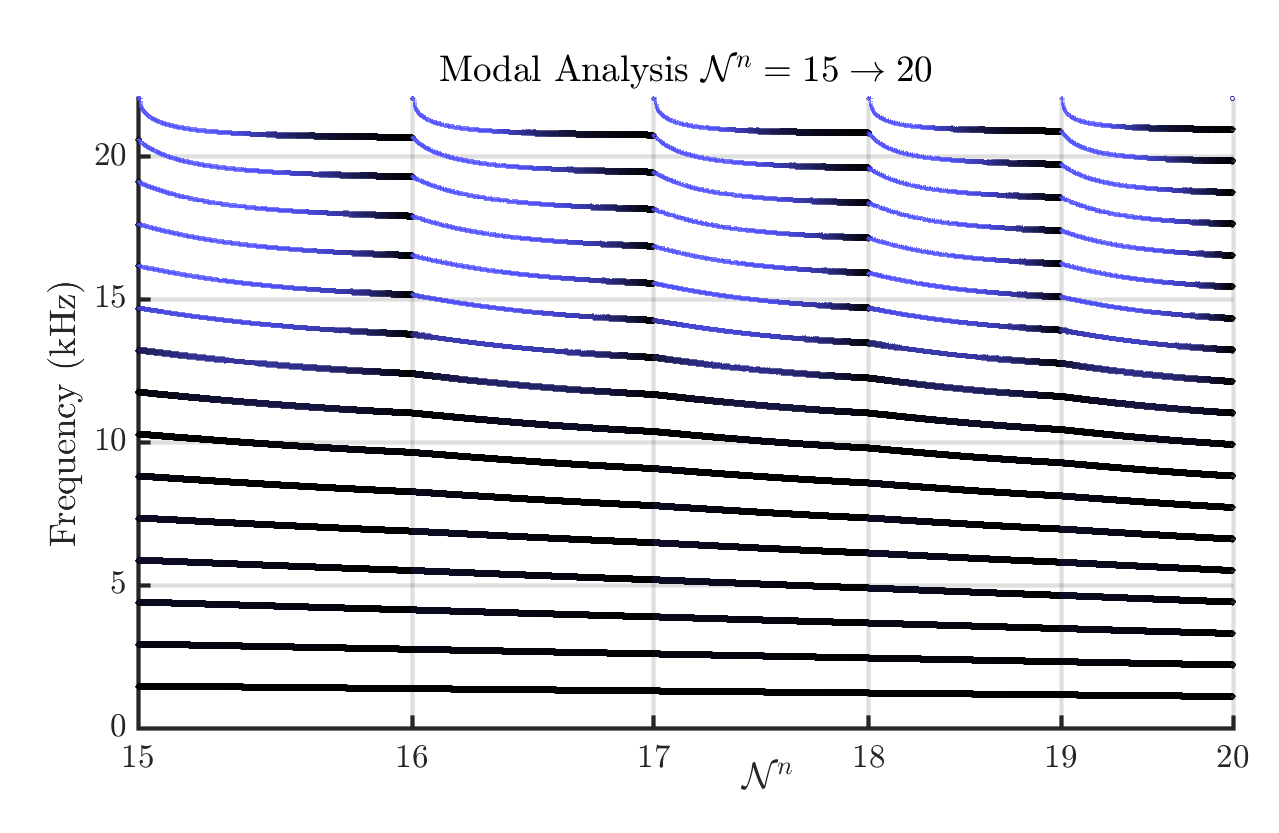
\includegraphics[width=0.8\textwidth]{figures/contributions/dynamicgrid/modalAnalysisOneStep.eps}\caption{Results of a modal analysis performed on the one-step form of the dynamic grid system in \eqref{eq:oneStepFormDynamicGrid}. Thinner and bluer lines indicate a higher amount of damping.\label{fig:modalAnalysisOneStep}}
\end{figure}

\begin{figure}[h]
    \centering
    \subfloat[$\Nfrac^n= 15 \rightarrow 20$, without displacement correction.]{\label{fig:specDown}{ 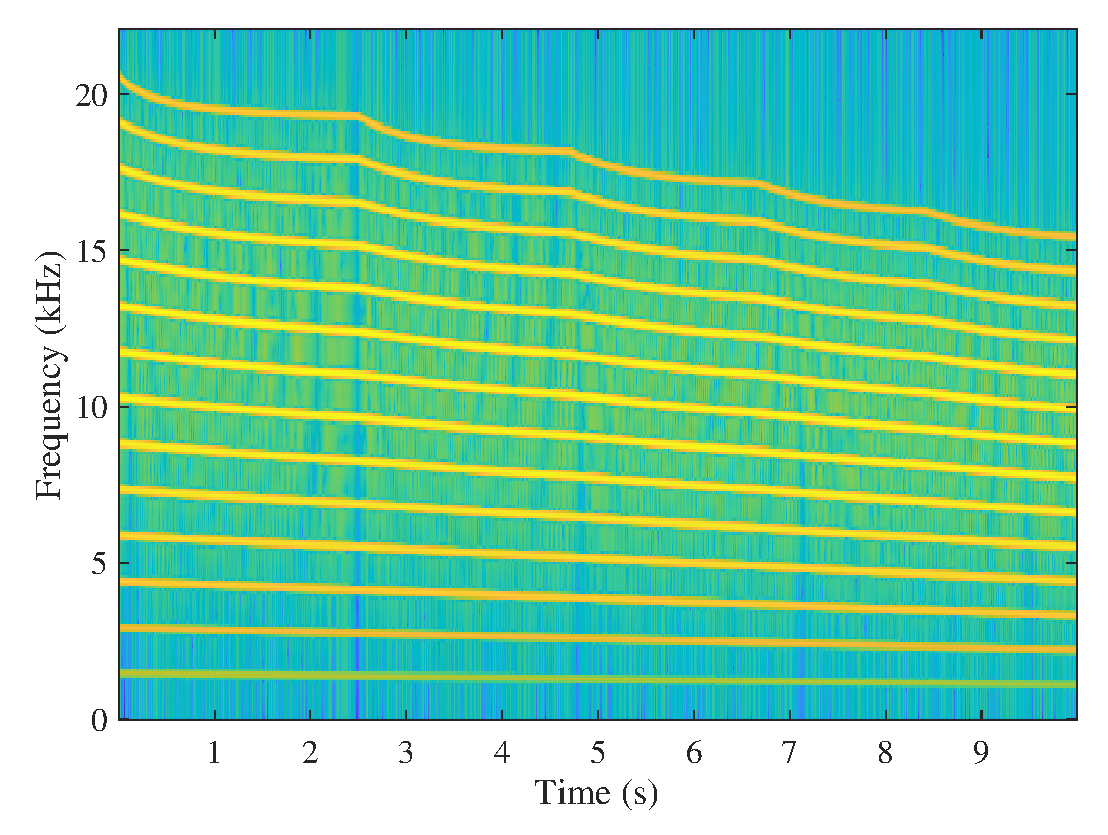
\includegraphics[width=0.45\textwidth]{figures/contributions/dynamicgrid/spectrogramDown.eps}}}
    \hfill
    \subfloat[$\Nfrac^n = 20 \rightarrow 15$, with displacement correction.]{\label{fig:specUp}{ 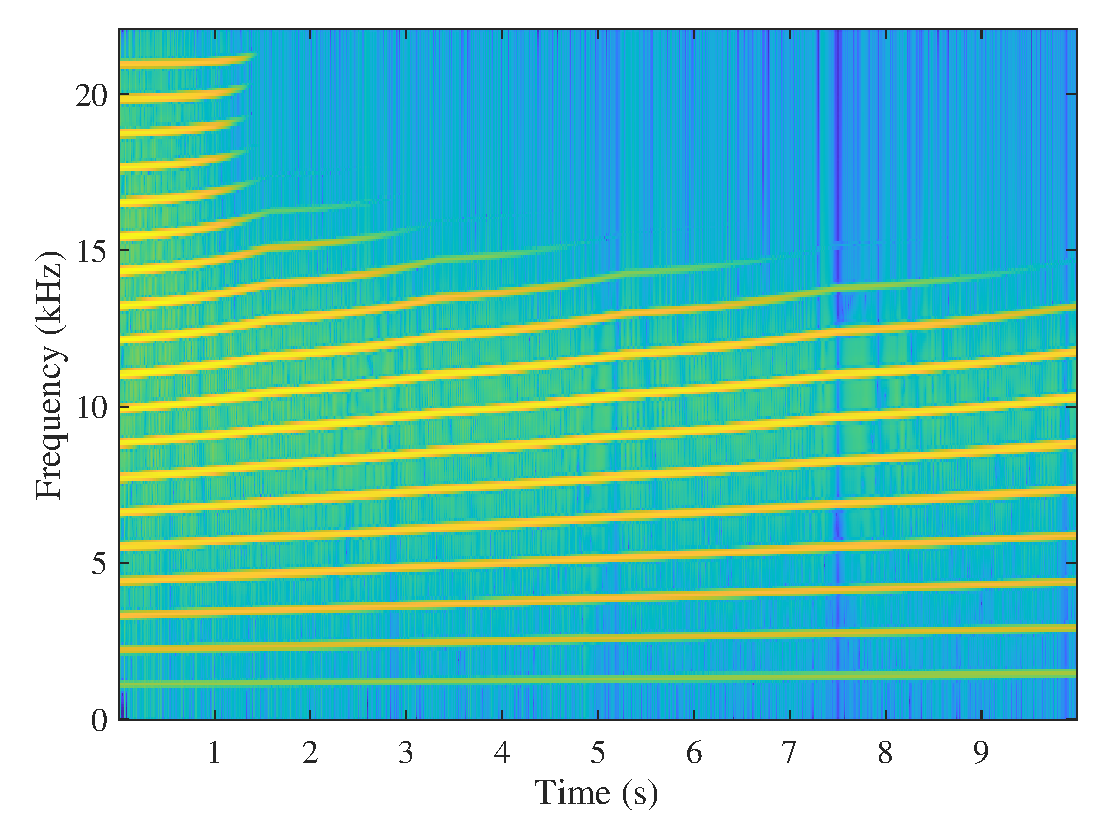
\includegraphics[width=0.45\textwidth]{figures/contributions/dynamicgrid/spectrogramUp.eps}}}
    \caption{Output spectra of an implementation of the dynamic grid.}\label{fig:specResults}
\end{figure}
\subsection{Modal analysis and results}\label{sec:modalAnalysisQuadDynamic}
Although the modal analysis techniques presented in Section \ref{sec:modalAnalysis} are only accurate for LTI systems, they can still be applied in the case of slow (sub-audio rate) parameter variations to obtain useful information about the scheme behaviour. In the process of creating the proposed dynamic grid method, modal analysis was indeed a key component in determining whether the method yielded satisfactory results.  

One can perform a modal analysis on the scheme by writing Eq. \eqref{eq:dynamicMatrixForm}
in one-step form (see Section \ref{sec:oneStepForm}}), 
\begin{equation}\label{eq:oneStepFormDynamicGrid}
    \begin{bmatrix}
        \Ucal^{n+1}\\
        \Ucal^n
    \end{bmatrix} = 
    \underbrace{\begin{bmatrix}
        (\A^n)^{-1}\B^n & (\A^n)^{-1}\C^n\\
        \I_{\mathcal{M}^n} & \mathbf{0}
    \end{bmatrix}}_{\Q^n}
    \begin{bmatrix}
        \Ucal^n\\
        \Ucal^{n-1}
    \end{bmatrix},
\end{equation}
where $\mathbf{0}$ is a $\fullMn\times \fullMn$ matrix of zeros. \footnote{Notice that, in the definitions for $\A^n$ and $\C^n$, $\beta$ can go to infinity, when $\alpha = \varepsilon = 0$ through Eq. \eqref{eq:betaDef}. In this case, $\varepsilon$ is set to a tiny non-zero value to avoid undefined results.} 

% The modal analysis can be used to analyse the system while parameters are varied, to determine whether the behaviour of the system is satisfactory. 
Figure \ref{fig:modalAnalysisOneStep} shows the result of a modal analysis performed on the one-step form shown in Eq. \eqref{eq:oneStepFormDynamicGrid} according to Section \ref{sec:oneStepForm}. The split of the original system is done as close to the right boundary as possible, such that the number of intervals $M^n$ and $M_w^n$ are calculated using Eq. \eqref{eq:alternativeM}. For a simulation lasting $n_\text{end}$ samples, the wave speed is varied linearly between $c^0 = 2940$, corresponding to $\Nfrac^0 = 15$, and $c^{n_\text{end}} = 2205$, corresponding to $\Nfrac^{n_\text{end}} = 20$. 

Figure \ref{fig:specResults} shows the output spectra of an implementation of the dynamic grid with the same parameter variation as used for the modal analysis. Figure \ref{fig:specDown} presents the spectral output of an implementation, where $\Nfrac = 20 \rightarrow 15$ without displacement correction, and shows that the modes follow the pattern predicted by the analysis. Figure \ref{fig:specUp} presents the spectral output where $\Nfrac = 15 \rightarrow 20$ with displacement correction activated. Although high-frequency modes get damped by the displacement correction, no artefacts are visible when changing grid configurations. Furthermore, the modes follow the pattern predicted by the modal analysis in reverse (as expected).

\subsection{Discussion and conclusion}\label{sec:conclusion}
% This section provides a brief summary of the results shown in paper \citeP[G]. 

Overall, the method satisfies the requirements detailed in the paper. The fundamental frequency of the system follows Eq. \eqref{eq:fundamentalFreq} with only very small deviations, as desired. Although larger deviations occur for higher frequency modes, these are not substantial. Looking at Figure \ref{fig:specUp}, the displacement correction seems to successfully prevent artefacts, but proper listening tests will need to be carried out to confirm this.

The results show that drawbacks of the method, such as frequency deviations and damping due to the displacement correction, mainly happen in higher frequency regions. As these are less relevant than lower frequencies due to the reasons presented in \citeP[G], the method can be concluded to work satisfactory. A more detailed discussion of the results can be found in the paper.  

One important aspect that is still missing from the presented method, is under what conditions it is stable. As stated in \cite{theBible}, stability for time-varying schemes are difficult to show using the current energy analysis framework (presented in Section \ref{sec:energyAnalysis}). The first step would be to perform a \textit{frozen coefficient analysis} \cite{Strikwerda1989}. In the case of this method, this means to fix $c^n$ at different values and prove stability in those cases. Finding these conditions has been left for future work, but would be a logical next step in the development of the dynamic grid method.

Other future work includes to extend the method to other systems, such as stiff strings (Chapter \ref{ch:stiffString}) or even 2D systems such as membranes and plates (Chapter \ref{ch:2Dsyst}). An interesting use case for this method is that of nonlinear systems, such as the Kirchhoff-Carrier string model \cite{Carrier1945} where parameters are varied based on the state of the system. 

\section{Interpolation experiments}\label{sec:iterations}
This section presents the results of experiments using different orders of interpolation to calculate the virtual grid points at the inner boundaries of the system, and aims to provide insight as to why quadratic interpolation has been chosen in the end. 

Four different Lagrangian interpolators are presented, ranging from linear to quartic (fourth order), and are made using the Lagrange interpolation formula in Eq. \eqref{eq:lagrangeForm}. Different orders of interpolation are included in the method by changing the definitions of the virtual grid points given in Eq. \eqref{eq:connectionInterpol}, and thereby the definition of the $\B^n$ matrix in Eq. \eqref{eq:quadMat}. As the effect of the displacement correction on the modal frequencies is negligible, this is excluded for clarity. Equation \eqref{eq:dynamicMatrixForm} can then be rewritten to 
\begin{equation}
    \Ucal^{n+1} = \B^n \Ucal^n- \Ucal^{n-1}
\end{equation}
and, using a test solution $\Ucal^n = z^n\boldPhi$ (following Section \ref{sec:modalAnalysis}), the eigenfrequencies can be calculated according to (using trigonometric identity \eqref{eq:cosIdentity})
\begin{equation}\label{eq:noDampModalAnalysis}
    f_p^n = \frac{1}{2 \pi k}\cos^{-1}\left(\frac{1}{2}\text{eig}_p(\B^n)\right).
\end{equation}

In the following, results will be shown for a varying wave speed corresponding $\Nfrac^n = 15 \rightarrow 20$, as was done in Section \ref{sec:modalAnalysisQuadDynamic}, but using Eq. \eqref{eq:noDampModalAnalysis}. For each interpolator, the case where the original system is split in the middle using Eq. \eqref{eq:addingPoint}, and where the split is at the right boundary using Eq. \eqref{eq:alternativeAddingPoint}, are considered. The black and red colours used in the figures do not carry extra meaning, and are only used for clarity of the plots. The results will be discussed at the end of this section. 
 
\subsubsection{Linear interpolation}
One can implement linear interpolation by changing the definitions in Eq. \eqref{eq:connectionInterpol} to
\begin{subequations}\label{eq:linearConnInterpol}
    \begin{align}
            u_{M^n+1}^n &= \alpha w_0^n + (1-\alpha)w_1^n,\label{eq:linearVirtU}\\
            w_{-1}^n &= (1-\alpha)u_{M^n-1}^n + \alpha u_{M^n}^n,
    \end{align}
\end{subequations}
such that the value of the virtual grid points of one system are fully defined by values of the other. 
% \def\pointFigWidth{0.8}
% \begin{figure}[h]
%     \centering
%     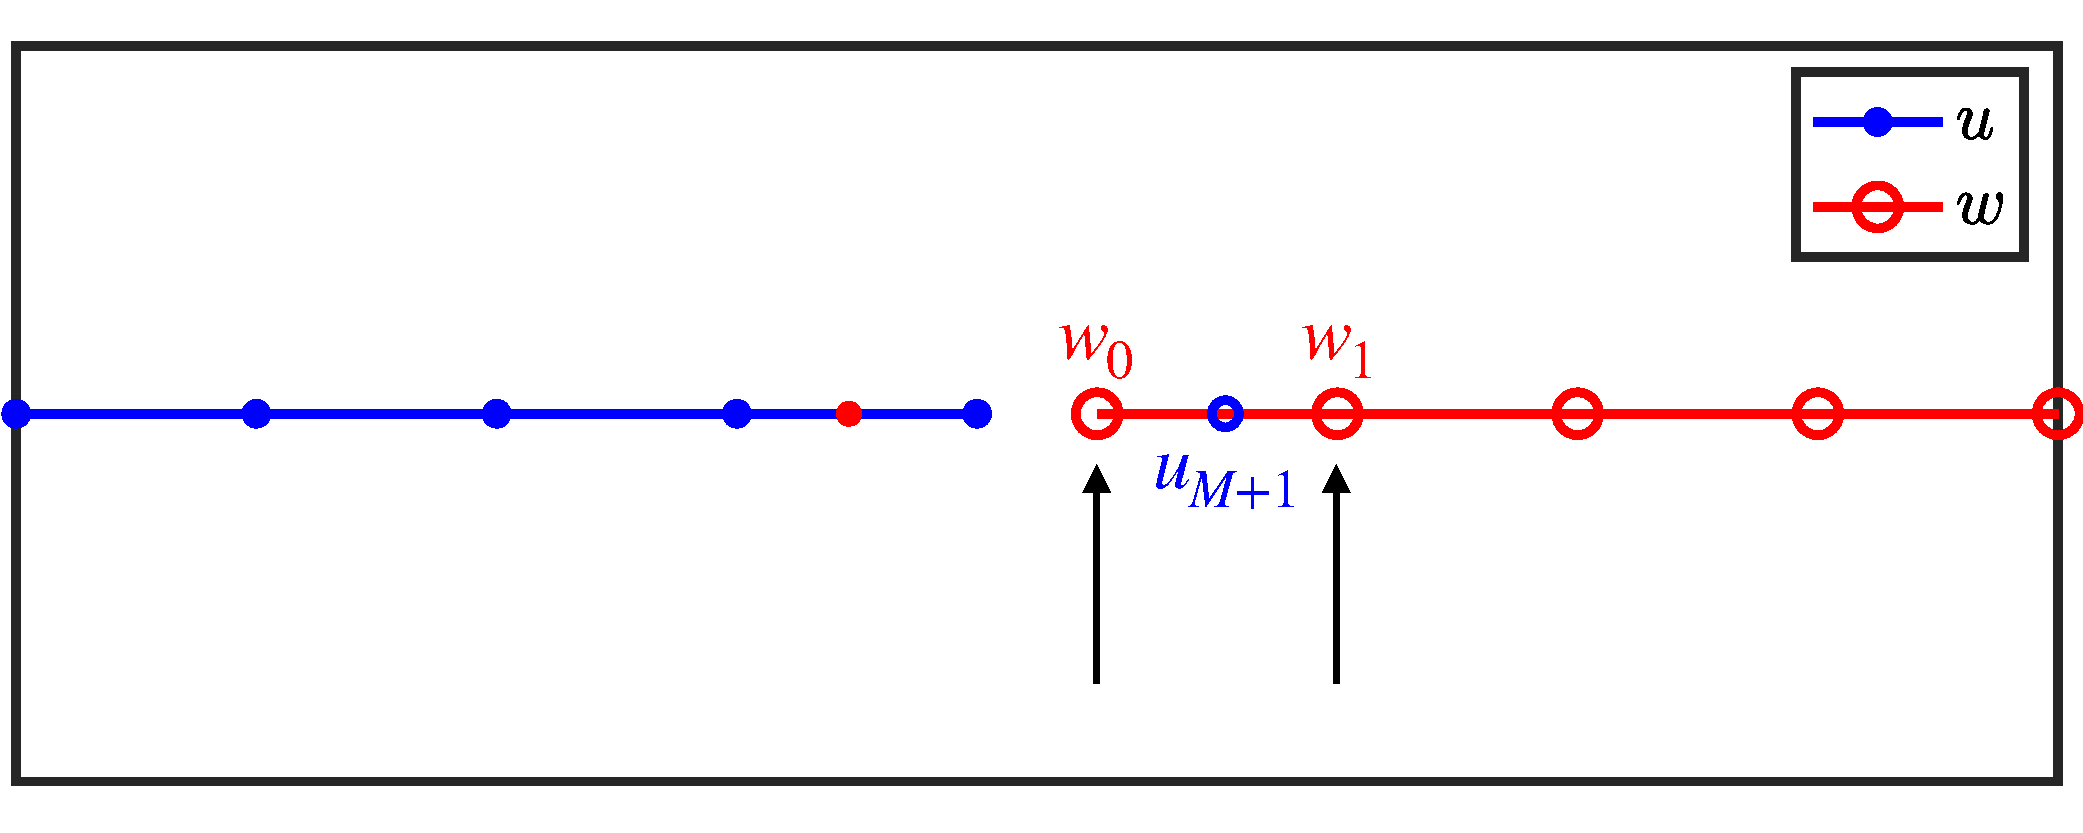
\includegraphics[width=\pointFigWidth\textwidth]{figures/contributions/dynamicgrid/interpolation/linearPoints.pdf}
%     \caption{Points used to calculate $u_{M^n+1}^n$ in Eq. \eqref{eq:linearVirtU}.
%     }
% \end{figure}

The $\B$ matrix in Eq. \eqref{eq:quadMat} can be changed to
\begin{equation}
    \B^n = \begin{bmatrix}[cccc|cccc]
     & \ddots  &\ddots & & & & 0 & \\
       & 1 & 0 & 1 & & & & \\
      & & 1 & 0 & \alpha & (1-\alpha) & \\ \cline{2-7}
      & & (1-\alpha) & \alpha &0 & 1 & & \\
         & & & &1 & 0 & 1  \\
         & 0 & &  &  &\ddots & \ddots &
    \end{bmatrix}
\end{equation}
and results are shown in Figure \ref{fig:linInterpRes}.
\begin{figure}[h]
    \centering
    \subfloat[Split is in middle.]{\label{fig:linearModesAddInCenter}{ 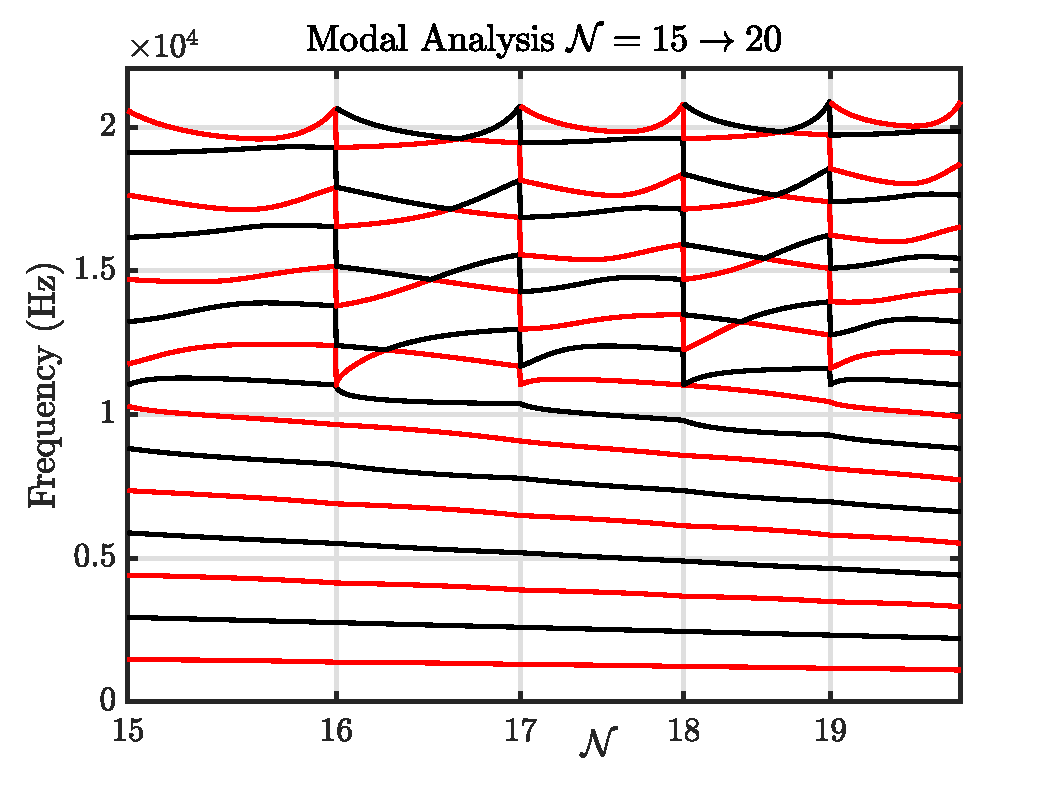
\includegraphics[width=0.49\textwidth]{figures/contributions/dynamicgrid/interpolation/linearMid.eps}}}
    \hfill
    \subfloat[Split is close to the boundary.]{\label{fig:linearModesAddBoundary}{ 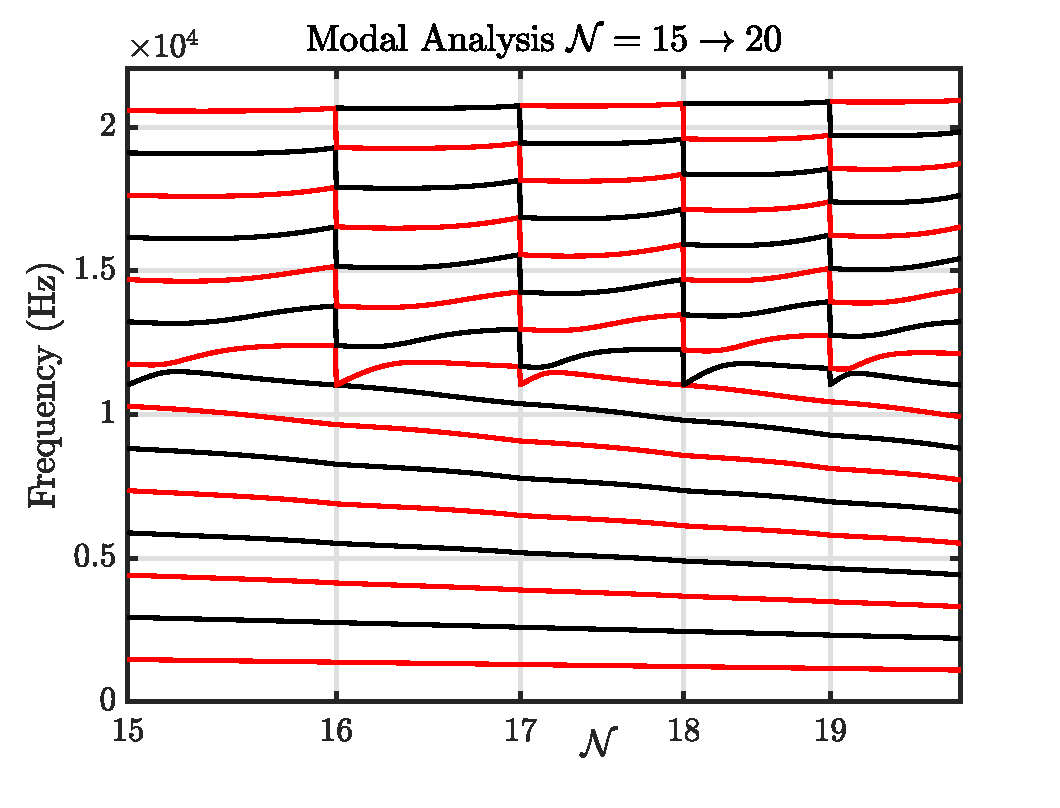
\includegraphics[width=0.49\textwidth]{figures/contributions/dynamicgrid/interpolation/linear1.eps}}}
    \caption{Results of modal analysis for linear interpolation.}\label{fig:linInterpRes}
\end{figure}

\subsubsection{Quadratic interpolation}
As quadratic interpolation is what the dynamic grid method is based on, no new definitions for Eqs. \eqref{eq:connectionInterpol} and \eqref{eq:quadMat} have to be given.
%
% \begin{figure}[h]
%     \centering
%     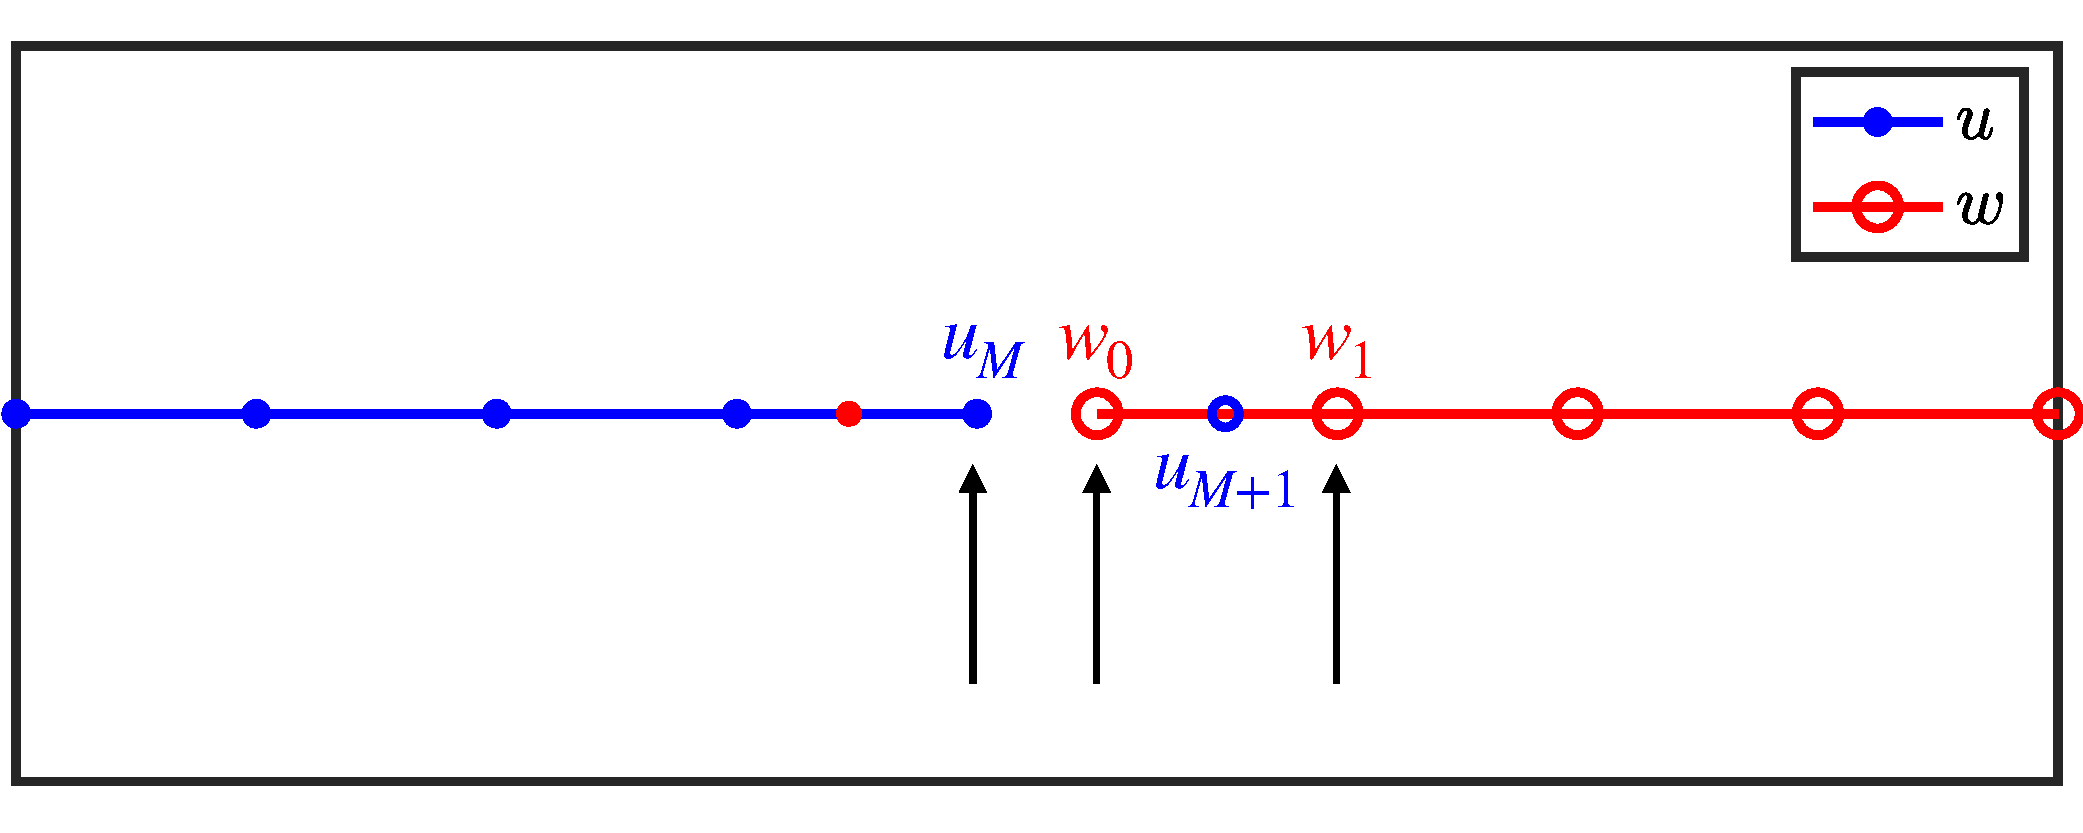
\includegraphics[width=\pointFigWidth\textwidth]{figures/contributions/dynamicgrid/interpolation/quadraticPoints.pdf}
%     \caption{Points used to calculate $u_{M^n+1}^n$ in Eq. \eqref{eq:calcUMP1}.\label{fig:quadraticPoints}}
% \end{figure}
%
Results of the modal analysis using Eq. \eqref{eq:noDampModalAnalysis} are shown in Figure \ref{fig:quadInterpRes}.

\begin{figure}[h]
    \centering
    \subfloat[Split is in middle.]{\label{fig:quadModesAddInCenter}{ 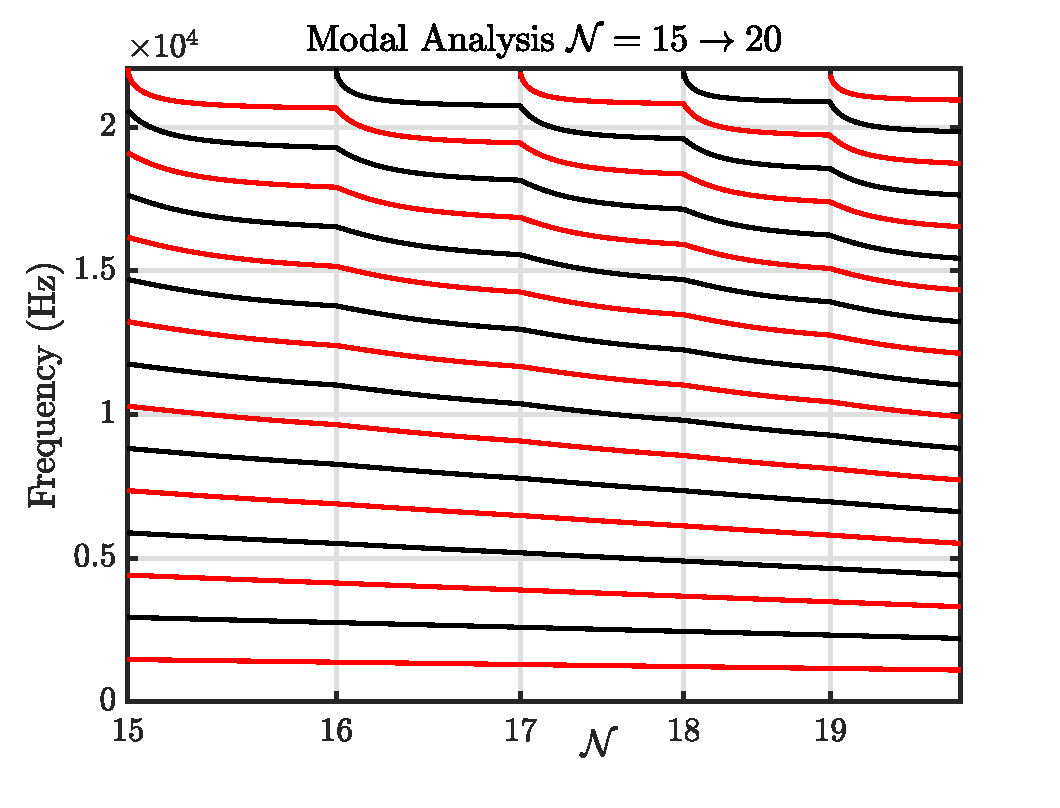
\includegraphics[width=0.49\textwidth]{figures/contributions/dynamicgrid/interpolation/quadMid.eps}}}
    \hfill
    \subfloat[Split is close to the boundary.]{\label{fig:quadModesAddBoundary}{ 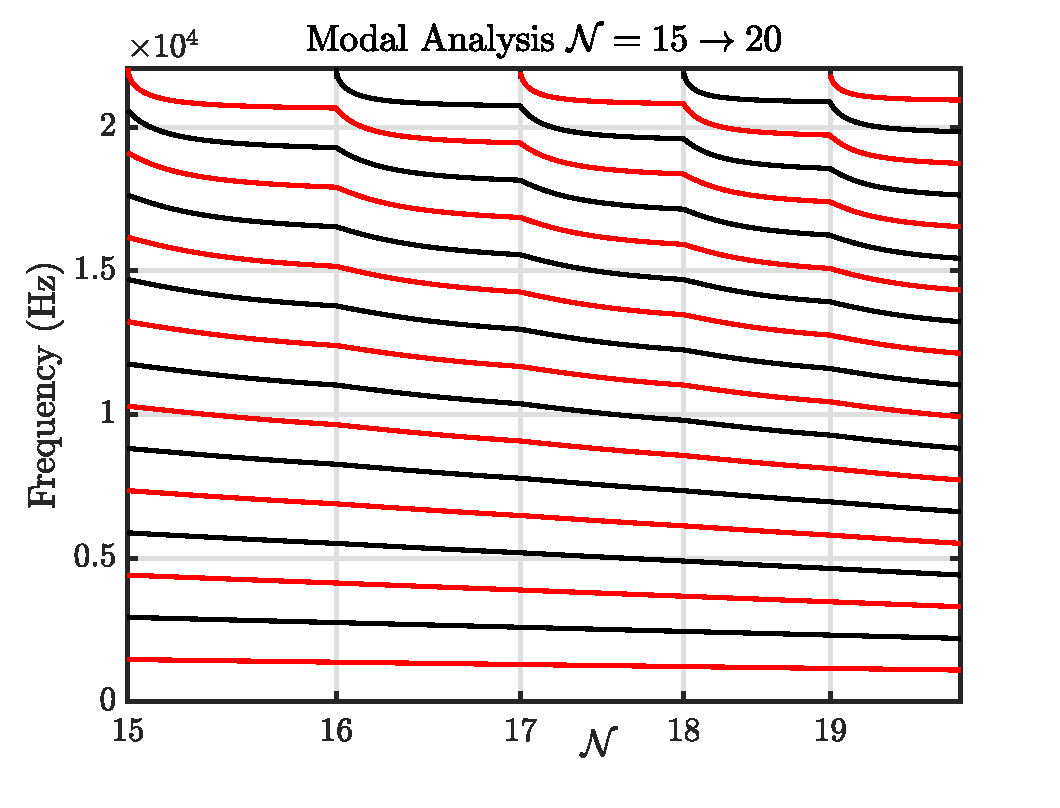
\includegraphics[width=0.49\textwidth]{figures/contributions/dynamicgrid/interpolation/quad1.eps}}}
    \caption{Results of modal analysis for quadratic interpolation.}\label{fig:quadInterpRes}
\end{figure}

\subsubsection{Cubic interpolation}
A cubic interpolator, using two points at either side of the virtual grid point, can be created using the Lagrangian interpolation formula in Eq. \eqref{eq:lagrangeForm}. The locations to calculate $u_{M^n+1}$ will be set to
\begin{equation}
    \begin{aligned}
     x_0 &= x_{u_{M^n}} = 0, \\
     x_1 &= x_{w_0} = \alpha, \\
     x_2& = x_{w_1} = \alpha + 1, \\
     x_3 &= x_{w_2} = \alpha + 2,
    \end{aligned}
\end{equation}
and the virtual grid point is at
\begin{equation}
    x = x_{u_{M^n}+1} = 1.
\end{equation}
The definitions for the virtual grid points can then be shown to be
\begin{subequations}\label{eq:cubicVirtualGridpoints}
    \begin{align}
            &u_{M^n+1}^n = \frac{\alpha - 1}{\alpha + 2}u_{M^n}^n + \frac{\alpha + 1}{2}w_0^n + (1-\alpha)w_1^n + \frac{\alpha (\alpha - 1)}{2(\alpha+2)}w_2^n,\\
            &w_{-1}^n = \frac{\alpha (\alpha - 1)}{2(\alpha+2)}u_{M^n-2}^n + (1-\alpha) u_{M^n-1}^n + \frac{\alpha+1}{2} u_{M^n}^n+ \frac{\alpha - 1}{\alpha + 2}w_{0}^n,
    \end{align}
\end{subequations}
and the $\B^n$ matrix can be set accordingly. 

If Eq. \eqref{eq:alternativeM} is used, and the split is placed close to the right boundary, the Dirichlet condition at this boundary needs to be extended to be simply supported, such that $w_2^n = -w_0^n$. As the value at the boundary remains $0$, i.e., $w_1 = 0$, this alters Eqs. \eqref{eq:cubicVirtualGridpoints} to be
\begin{align*}
    &u_{M^n+1}^n = \frac{\alpha - 1}{\alpha + 2}u_{M^n}^n + \left(\frac{\alpha + 1}{2}-\frac{\alpha (\alpha - 1)}{2(\alpha+2)}\right)w_0^n\\
    &w_{-1}^n = \frac{\alpha (\alpha - 1)}{2(\alpha+2)}u_{M^n-2}^n + (1-\alpha) u_{M^n-1}^n + \frac{\alpha+1}{2} u_{M^n}^n.
\end{align*}
The results are shown in Figure \ref{fig:cubicInterpRes}.
\begin{figure}[h]
    \centering
    \subfloat[Split is in middle.]{\label{fig:cubicModesAddInCenter}{ 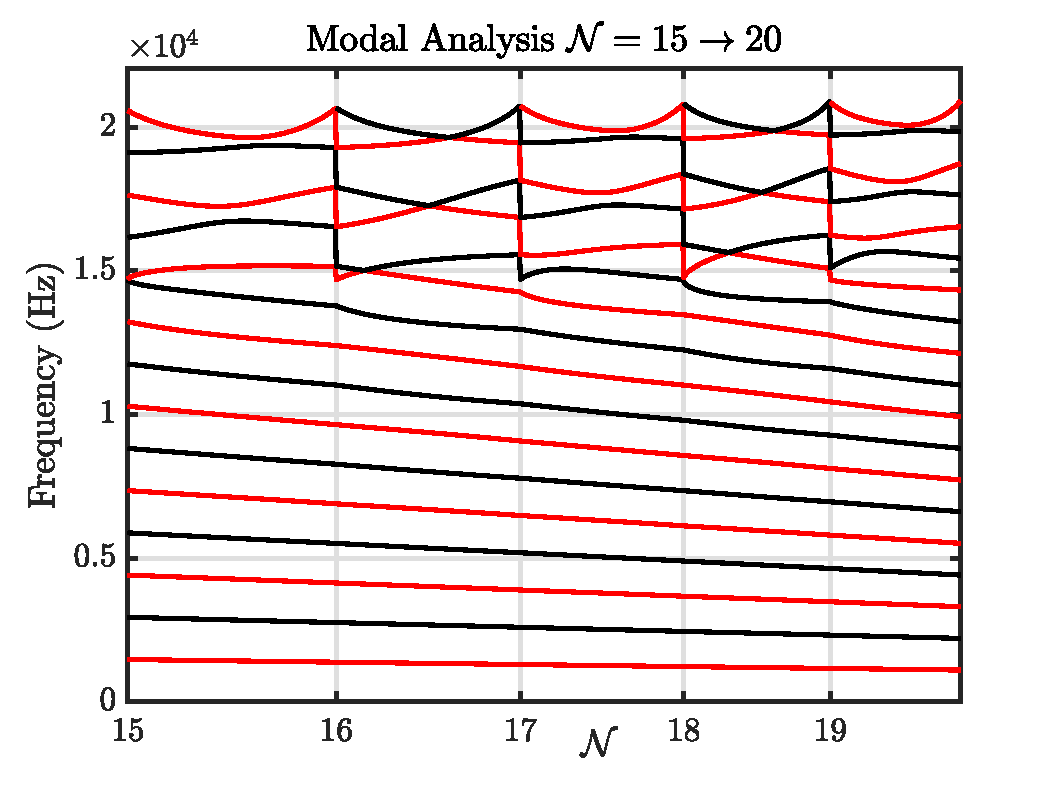
\includegraphics[width=0.49\textwidth]{figures/contributions/dynamicgrid/interpolation/cubicMid.eps}}}
    \hfill
    \subfloat[Split is close to the boundary.]{\label{fig:cubicModesAddBoundary}{ 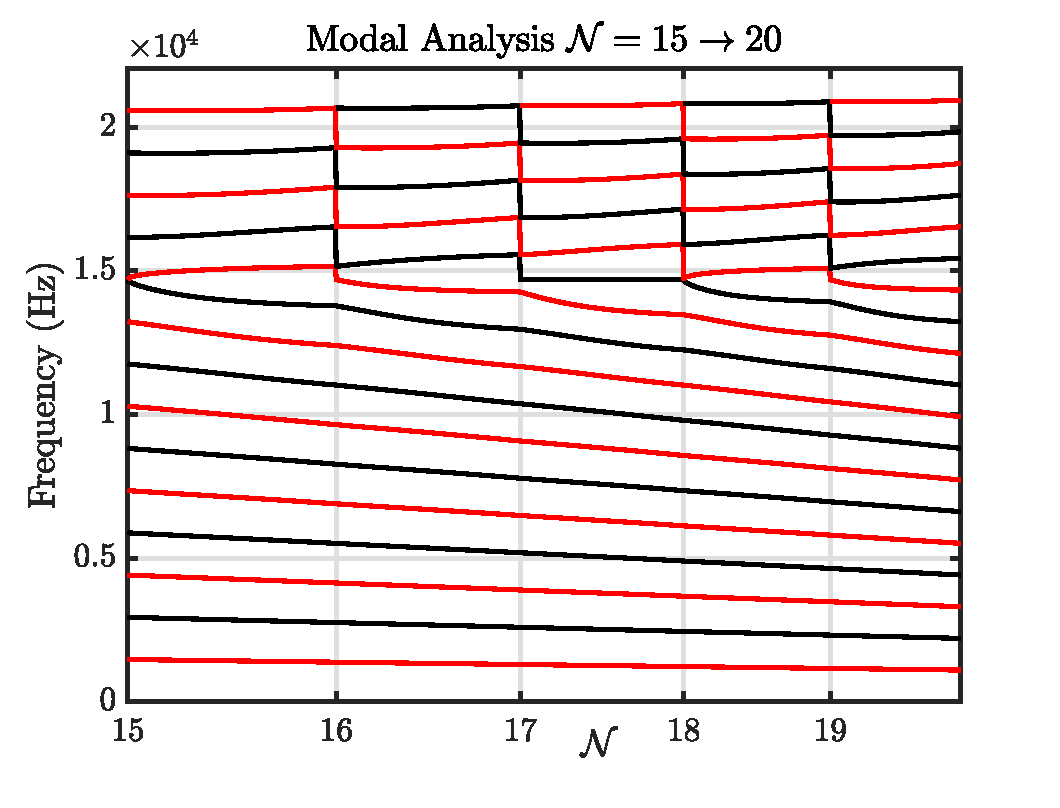
\includegraphics[width=0.49\textwidth]{figures/contributions/dynamicgrid/interpolation/cubic1.eps}}}
    \caption{Results of modal analysis for cubic interpolation.}\label{fig:cubicInterpRes}
\end{figure}

\subsubsection{Quartic interpolation}
Finally, a quartic interpolator} can be created from Eq. \eqref{eq:lagrangeForm}. At the boundary, it can be implemented similar to the cubic interpolator. Results of a quartic interpolator can be found in Figure \ref{fig:quarticInterpRes}.

\begin{figure}[h]
    \centering
    \subfloat[Split is in middle.]{\label{fig:quarticModesAddInCenter}{ 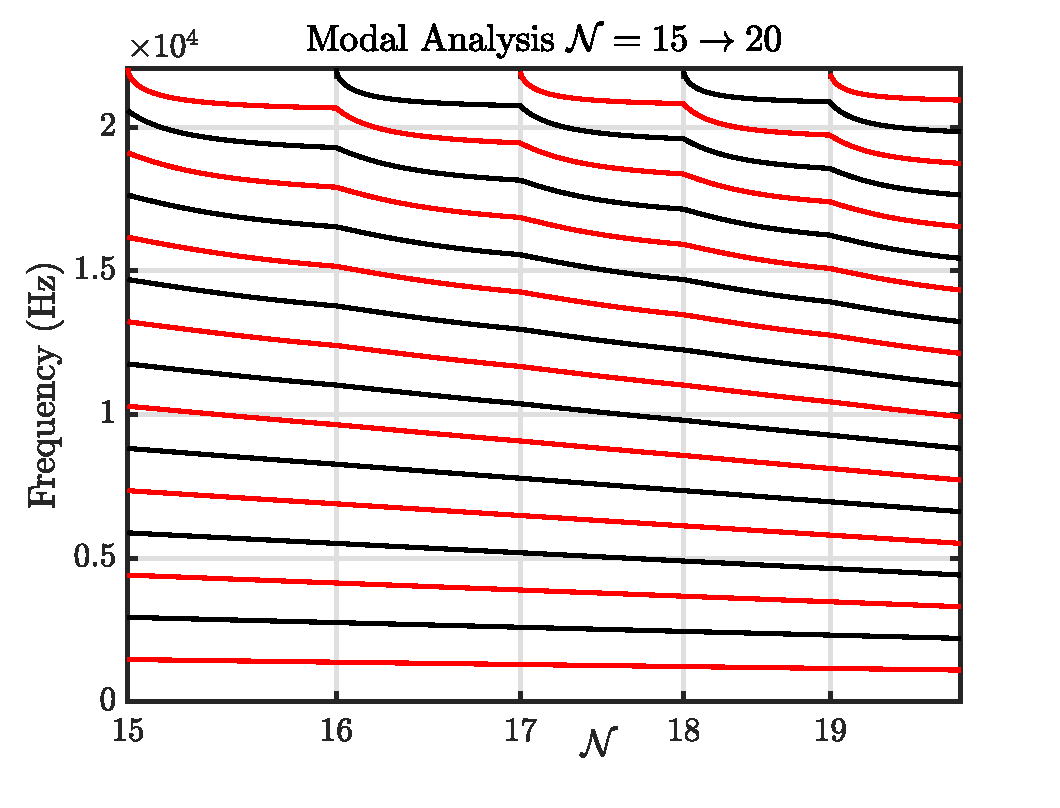
\includegraphics[width=0.49\textwidth]{figures/contributions/dynamicgrid/interpolation/quarticMid.eps}}}
    \hfill
    \subfloat[Points are added at close to the boundary.]{\label{fig:quarticModesAddBoundary}{ 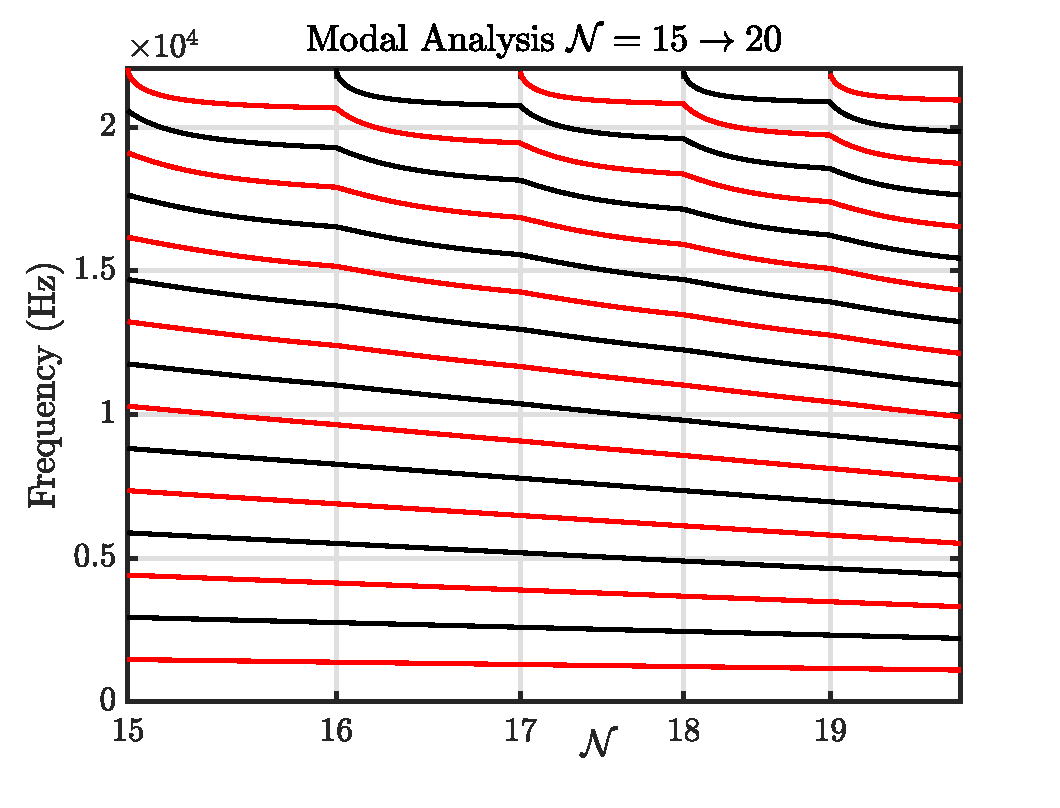
\includegraphics[width=0.49\textwidth]{figures/contributions/dynamicgrid/interpolation/quartic1.eps}}}
    \caption{Results of modal analysis for quartic (fourth-order) interpolation.}\label{fig:quarticInterpRes}
\end{figure}

\subsection{Discussion}
The results show a large behavioural difference between odd-ordered (linear, cubic) interpolators and even-ordered (quadratic, quartic) interpolators.  

Figure \ref{fig:linInterpRes} shows that for linear interpolation, modes with frequencies below $\fs/4$ Hz ($1/2$ the Nyquist frequency) move downwards as $\Nfrac^n$ increases, as expected, but modes above this frequency generally move upwards. If the split is in the middle, `modal crossings' appear for even values of $\floor[\Nfrac^n]$, but they do not occur when the split is close the boundary. Similar behaviour occurs for cubic interpolation in Figure \ref{fig:cubicInterpRes}, but the split happens around $3/8 \fs$ Hz ($3/4$ the Nyquist frequency). Again, adding points close to the boundary resolves the modal crossings. 

The modal patterns created by even-ordered interpolators, exhibit behaviour closer to what is desired (see Figures \ref{fig:quadInterpRes} and \ref{fig:quarticInterpRes}). All modal frequencies move down and no modal crossings occur. Interestingly, the even-ordered interpolators show no differences in their modal behaviour when the split is in the middle of the original system versus close to the boundary (the differences are within machine precision).

Frequency deviations happen to a lesser degree for the quartic interpolator than for the quadratic interpolator, and continue to decrease for higher-ordered (even) interpolators. The differences have been found negligible and as flexibility of the method decreases as the interpolation order increases (as more grid points are required for the virtual grid point calculation), the quadratic interpolator has been chosen in the eventual method. 

% The exact reasons for the results discussed in this section are yet to be discovered, although is safe to say that the differences between odd and even-ordered interpolators are related to differences in the matrix structure.\footnote{For example, matrices for even-ordered interpolators have ones along the diagonals next to the main diagonal for any value of $\alpha$.}

\section{Examples of use cases}\label{sec:examples}
This section provides several examples of instruments using dynamic parameter variations and can be used as inspiration for future work. As mentioned in paper \citeP[G], the interest lies in dynamic changes in the defining parameters of the resonator, as opposed to a pitch change using a fretting finger, for example. 
% Paper \citeP[H] presents the trombone (also see Chapter \ref{ch:trombone}) which is very interesting to model due to its time-varying geometry.

% The following cases of instruments using dynamic parameter variation and can be used as inspiration for future work. 

\subsubsection{1D systems}
A defining property that can physically be changed in strings is the tension. 
% Usually, pitch changes in guitar strings happen by pressing the string against the fretboard. 
There are various ways to smoothly change the pitch by changing the tension in the string. A straightforward way to do this would be to move the fretting finger perpendicular to the string while pressing down to create a pitch bend. Other, less common ways are to modulate the tension by pressing down on the small length of string between the tuning peg and the nut\footnote{John Mayer - Gravity (Live in L.A.): \url{https://youtu.be/dBFW8OvciIU?t=284}}, or turn the tuning pegs directly while playing.\footnote{Jon Gomm - Passionflower: \url{https://youtu.be/nY7GnAq6Znw?t=49}}\textsuperscript{,}\footnote{gr4yhound - servo bender: \url{https://youtu.be/fSQ9Dg65EFo}}

The hammered dulcimer is another example where the strings are placed over a bridge, where one can play the string at one side of the bridge, while pushing down on the same string on the other side.\footnote{Amazing Hammered Dulcimer Musician - Joshua Messick: \url{https://youtu.be/veuGTnzgNRU?t=215}}

Apart from strings, acoustic tubes also lend themselves to applications of the dynamic grid. The main example is the trombone as published in \citeP[H], where the method presented in this chapter is used. The slide whistle falls in the same category. 

\subsubsection{2D systems}
One could potentially extend the dynamic grid method presented here to 2D, and model physical tension changes in membranes. The membrane tension in timpani, for example, can be changed using a footpedal. The Bodhr\'an is a membranophone where the player hits the membrane on one side and can change the pitch by pressing on the other side.\footnote{John Joe Kelly Bodhran Solo - Christ church Dublin 2012: \url{https://youtu.be/b9HyB5yNS1A?t=146}} The pitch of a talking drum (hourglass drum) can be changed be squeezing the laces attached to the membrane.\footnote{Ayan Bisi Adeleke - Master talking drummer - drum talks: \url{https://youtu.be/B4oQJZ2TEVI?t=9}} An example of a pitch-modulated thin plate is the musical saw, where the curvature of the saw is changed to create different pitches.\footnote{Musical Saw performance by Sakita Hajime: \url{https://youtu.be/-6nv0iDrAis}}
%the `flex-a-tone' where one curves
%     \item Timpani
%     \item Bodhr\'an: https://youtu.be/b9HyB5yNS1A?t=146
%     \item Talking drum (hourglass drum): https://youtu.be/B4oQJZ2TEVI?t=9
%     \item Flex-a-tone (could also be 1D tbh..): https://www.youtube.com/watch?v=HEW1aG8XJQk.
% \end{itemize}




% Something about time-dependent variable coefficient Stokes flow:
% https://arxiv.org/abs/1010.2832

% Time-varying propagation speed in waveguides: https://quod.lib.umich.edu/cgi/p/pod/dod-idx/fractional-delay-application-time-varying-propagation-speed.pdf?c=icmc;idno=bbp2372.1997.069;format=pdf

% Special boundary conditions (look at!):
% Modeling of Complex Geometries and Boundary Conditions in Finite Difference/Finite Volume Time Domain Room Acoustics Simulation (\url{https://www.researchgate.net/publication/260701231_Modeling_of_Complex_Geometries_and_Boundary_Conditions_in_Finite_DifferenceFinite_Volume_Time_Domain_Room_Acoustics_Simulation})

